\documentclass[solution, letterpaper]{cs20inclass}
\usepackage{enumerate}
\usepackage{tikz}
\usepackage{pgf}
\usepackage{tikz}
\usepackage{hyperref}
\begin{document}
\header{16}{Friday, March 4, 2016}

\noindent Authors: Crystal Chang and Ben Zheng

\paragraph*{Executive Summary}
\begin{enumerate}

\item A \textbf{state machine} is a binary relation called a \textit{transition relation} on a set of elements $S$ called \textit{states}, visually depicted as nodes.
\begin{itemize}
\item A transition from state $q$ to $r$ is denoted $q \rightarrow r$.
\item A state machine has a start state $q_0 \in S$, which is denoted with an arrow pointing to the start state's node.
\item A state machine may have one or more final states, which are denoted with double-circles around the nodes of the final states.
\end{itemize}
\item An \textit{execution} of a state machine with a set of states $S$ is a plausible sequence of states (possibly an infinite one) with the property that
\begin{itemize}
\item the sequence starts with the start state $q_0 \in S$, and
\item for all consecutive states $q$ and $r$, $q \rightarrow r$.
\end{itemize}
\item A state $s \in S$ is \textit{reachable} if some execution of a state machine includes $s$.
\item Predicate $P$ is a preserved invariant of a state machine if for all $q,r \in S$,
$$P(q) \wedge (q \rightarrow r) \implies P(r)$$
\item \textbf{The Invariant Principle}: If a preserved invariant of a state machine is true for the start state, then it is true for all reachable states.
\item A state machine is \textit{deterministic} if for all states $s$ in the machine, there is at most one transition out of $s$.
\item A state machine is \textit{non-deterministic} if there exists a state $s$ in the machine such that there is more than one transition out of $s$.
\end{enumerate}

\pagebreak

%% PROBLEM 1 %%
\problem Draw a state machine with states, labelled transitions, start state, and final state(s) that accepts exactly
\subproblem the binary string $101$.
\subproblem binary strings that begin with the sequence $101$.
\subproblem binary strings that begin and end with $1$ (i.e. $1, 11, 101, 111,\ldots$).
\subproblem no strings (the empty set).

\begin{solution}
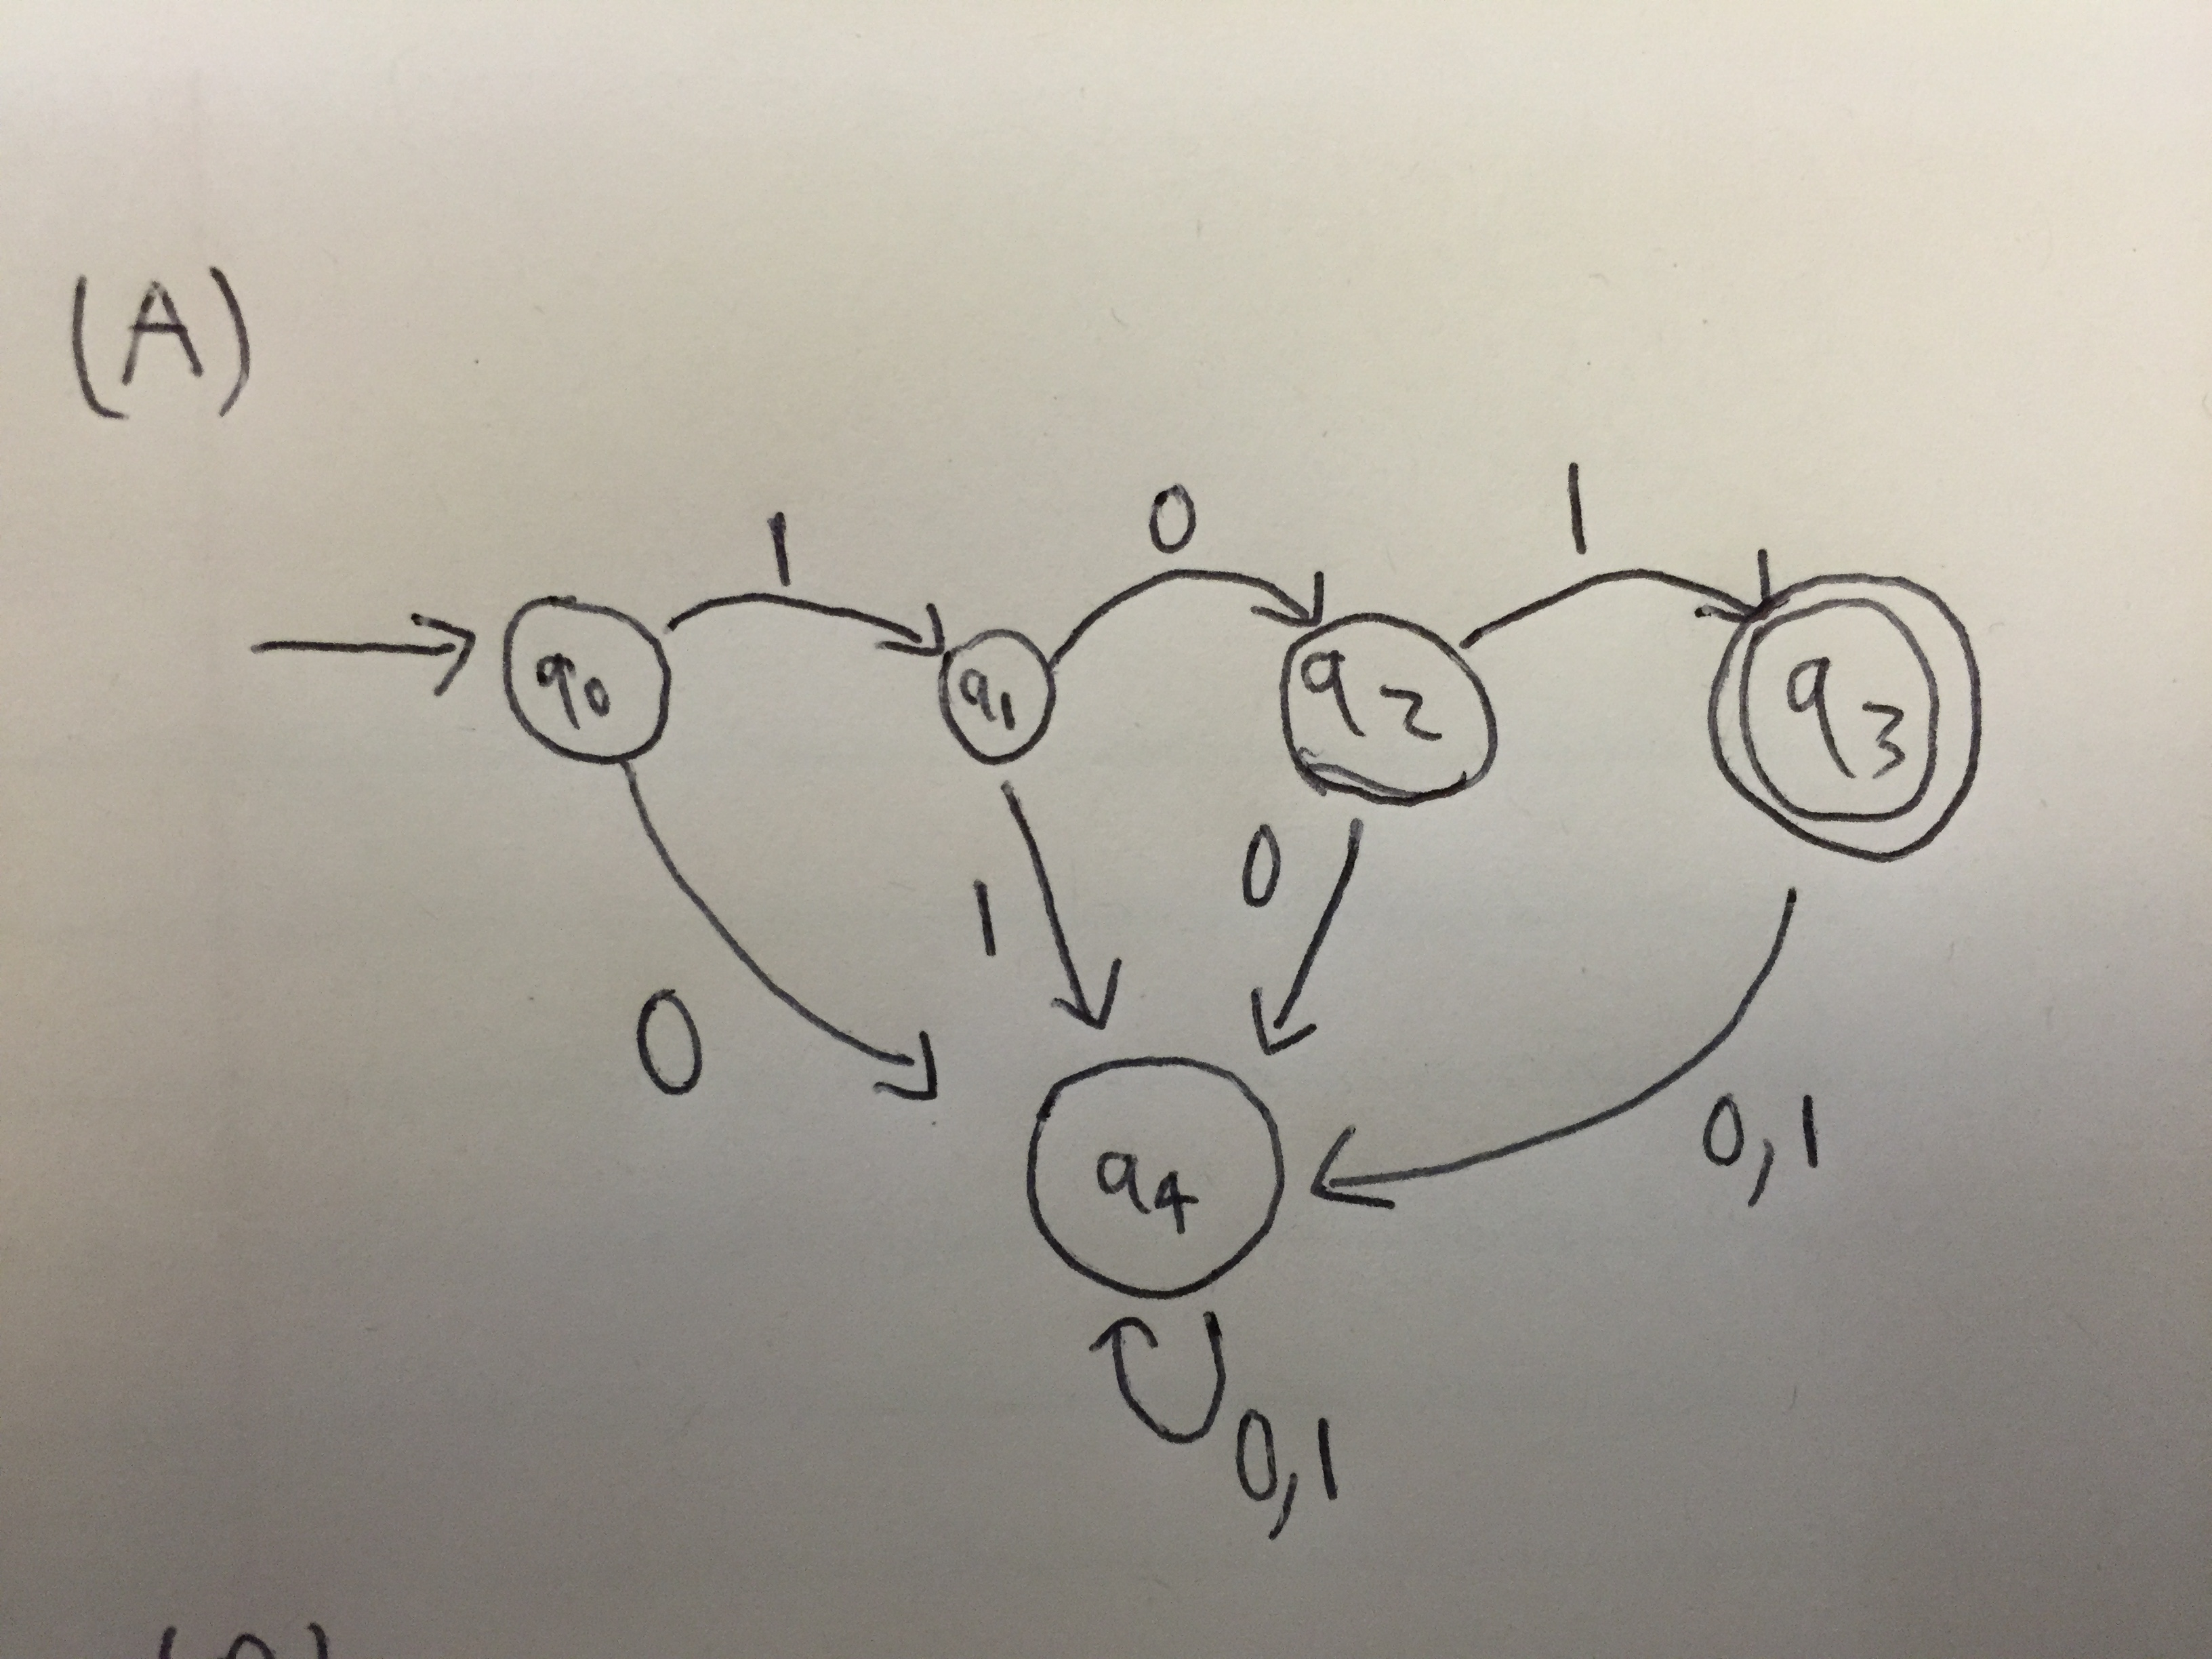
\includegraphics[width=15cm]{class16p1a}


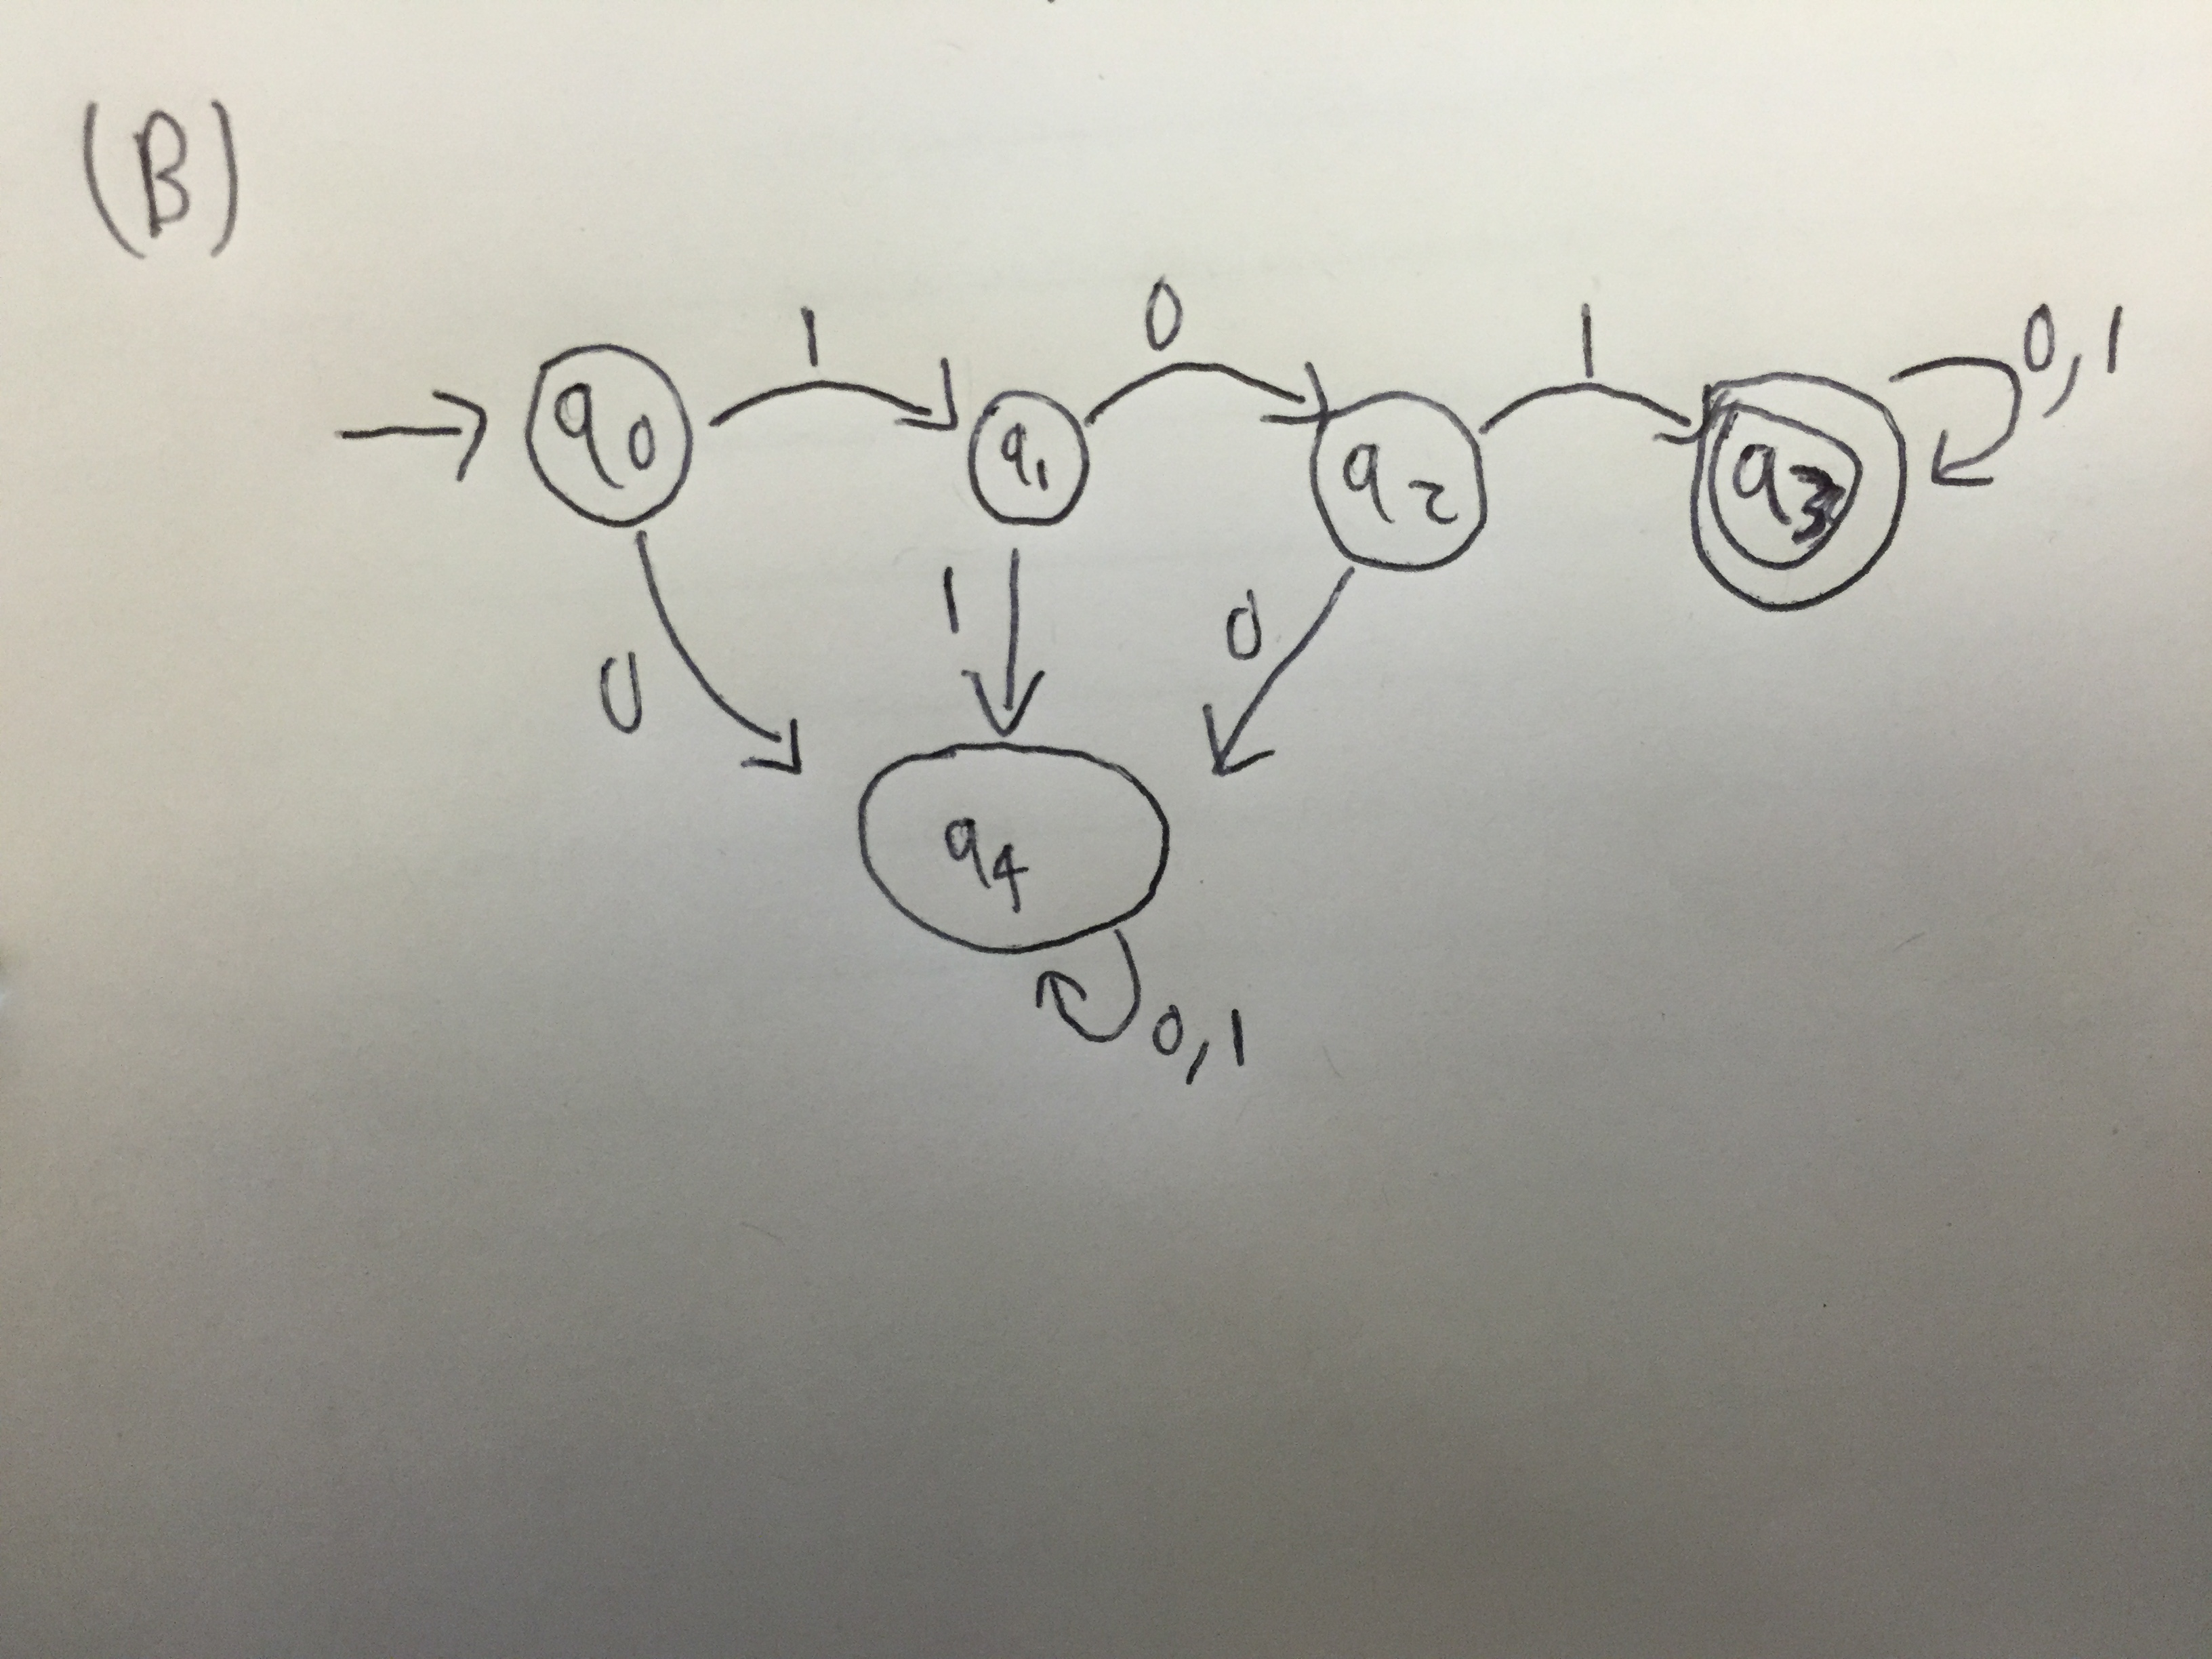
\includegraphics[width=15cm]{class16p1b}


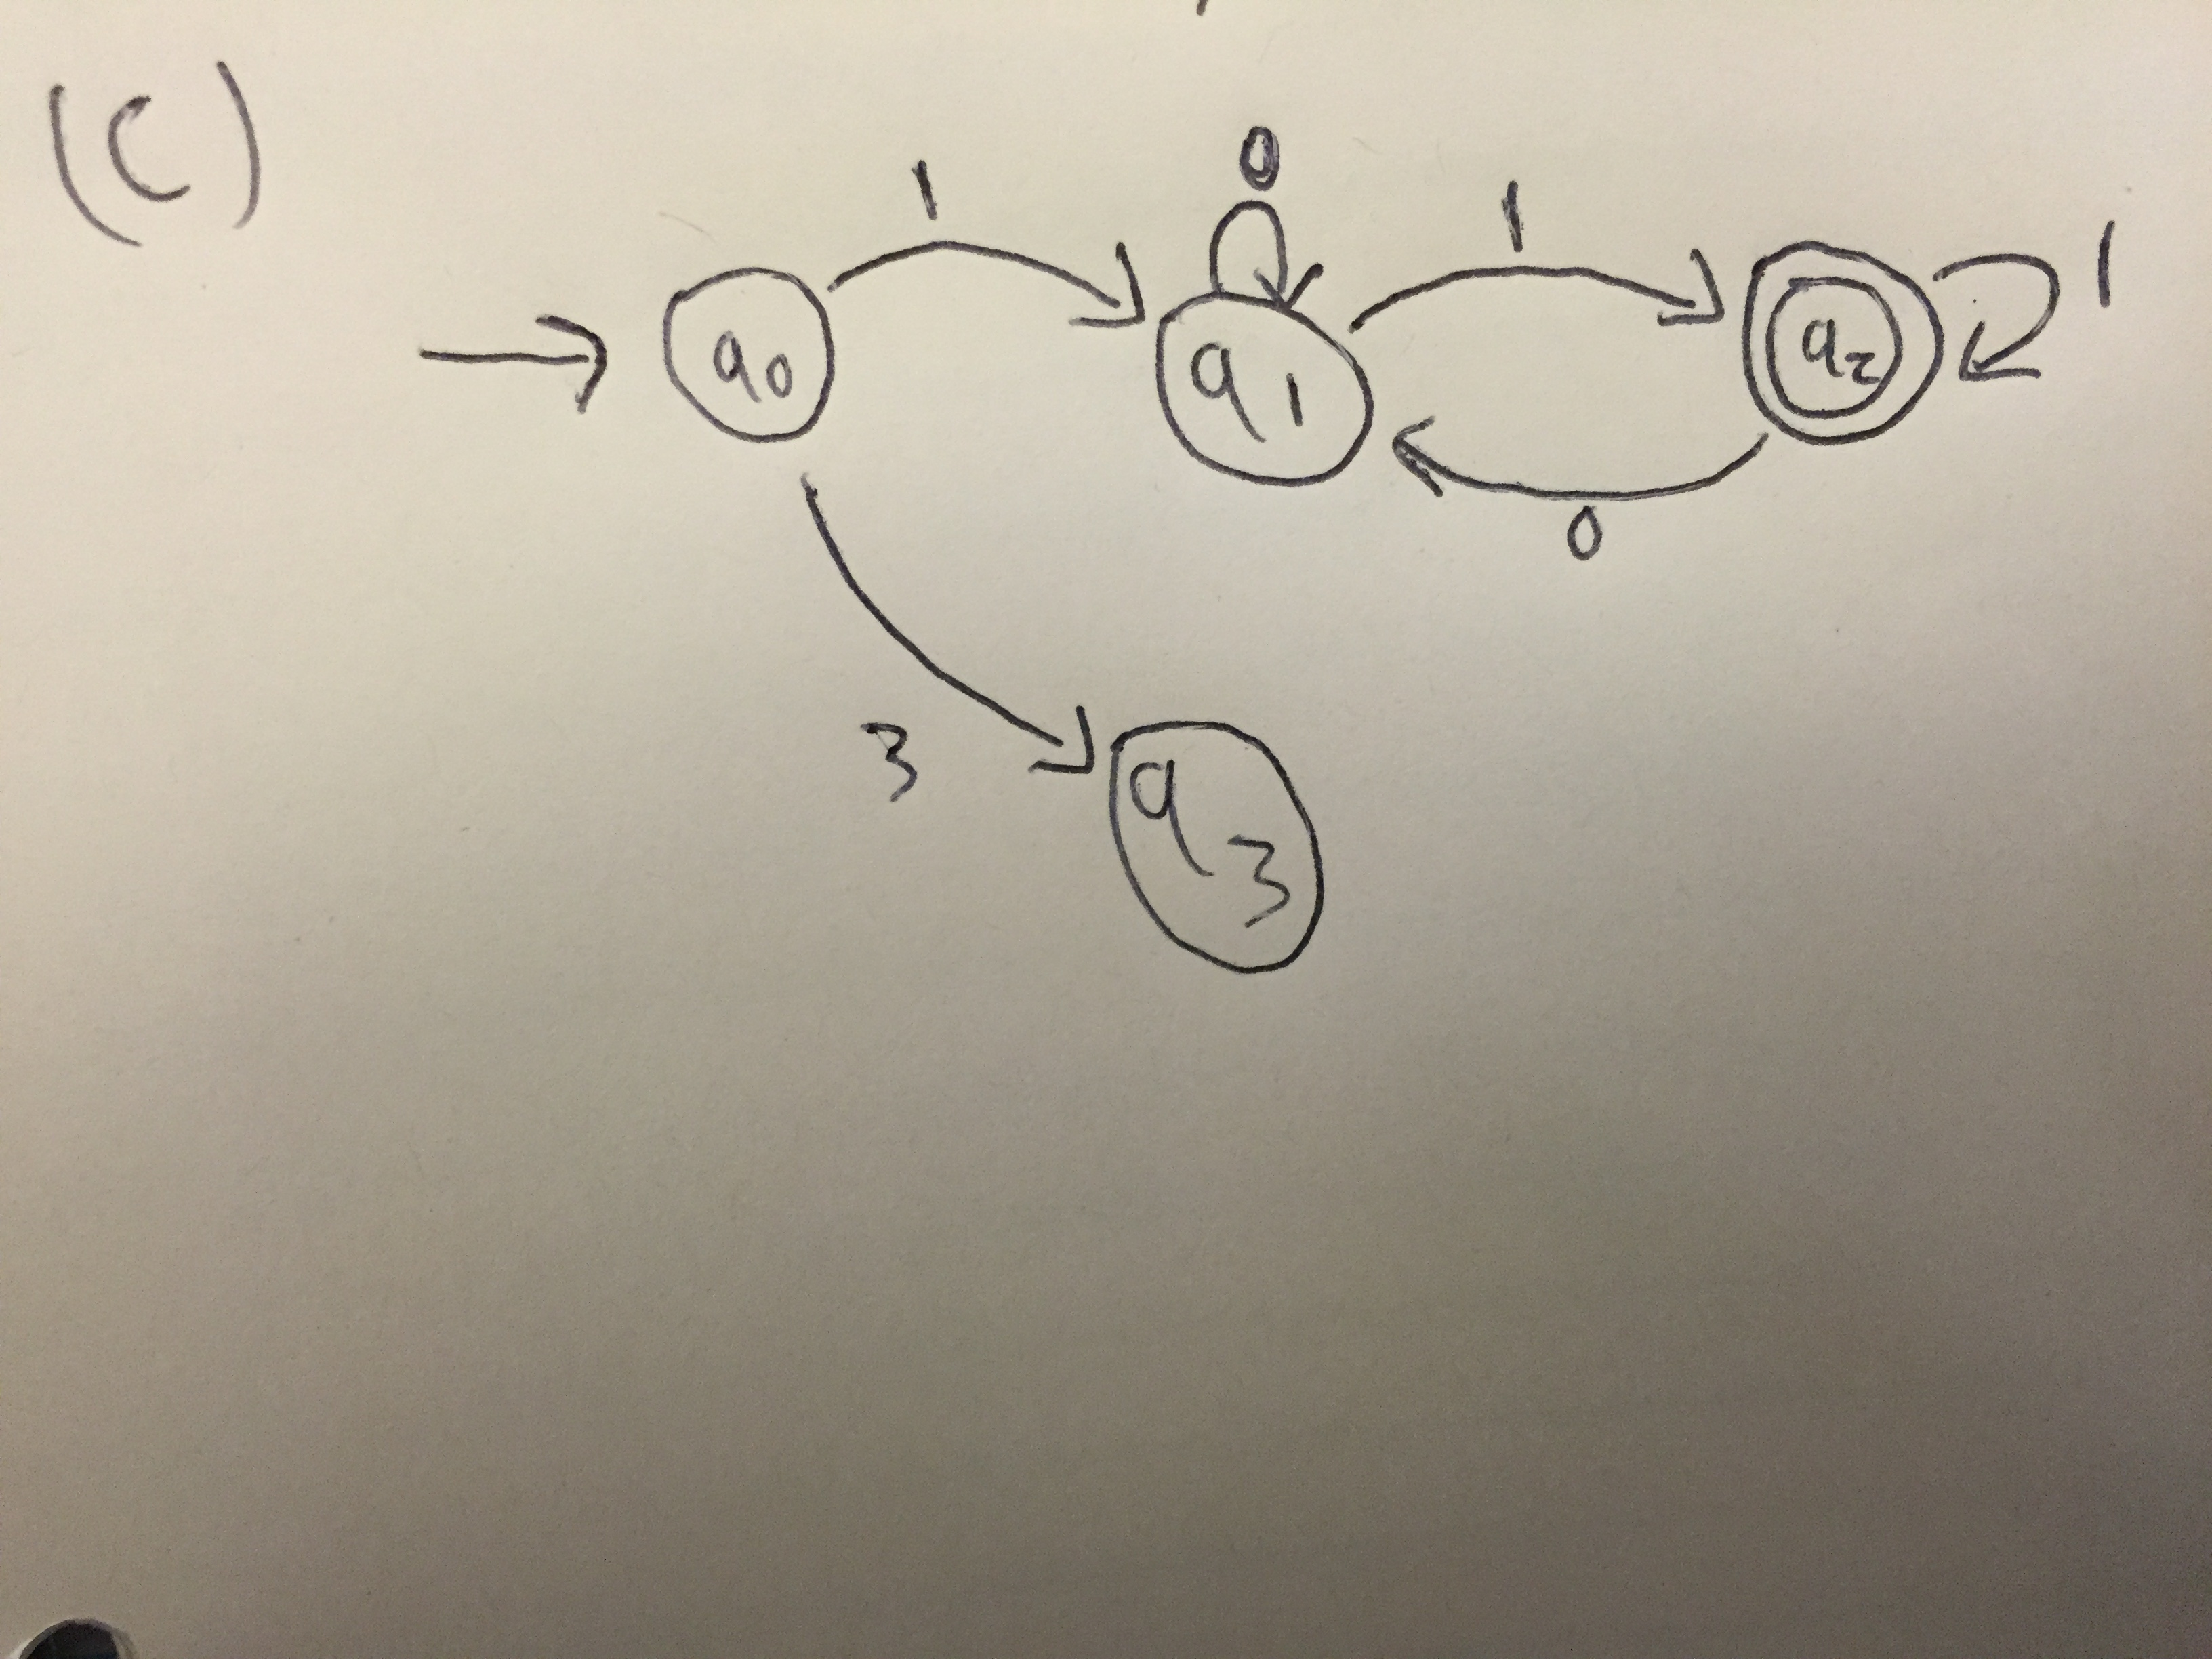
\includegraphics[width=15cm]{class16p1c}


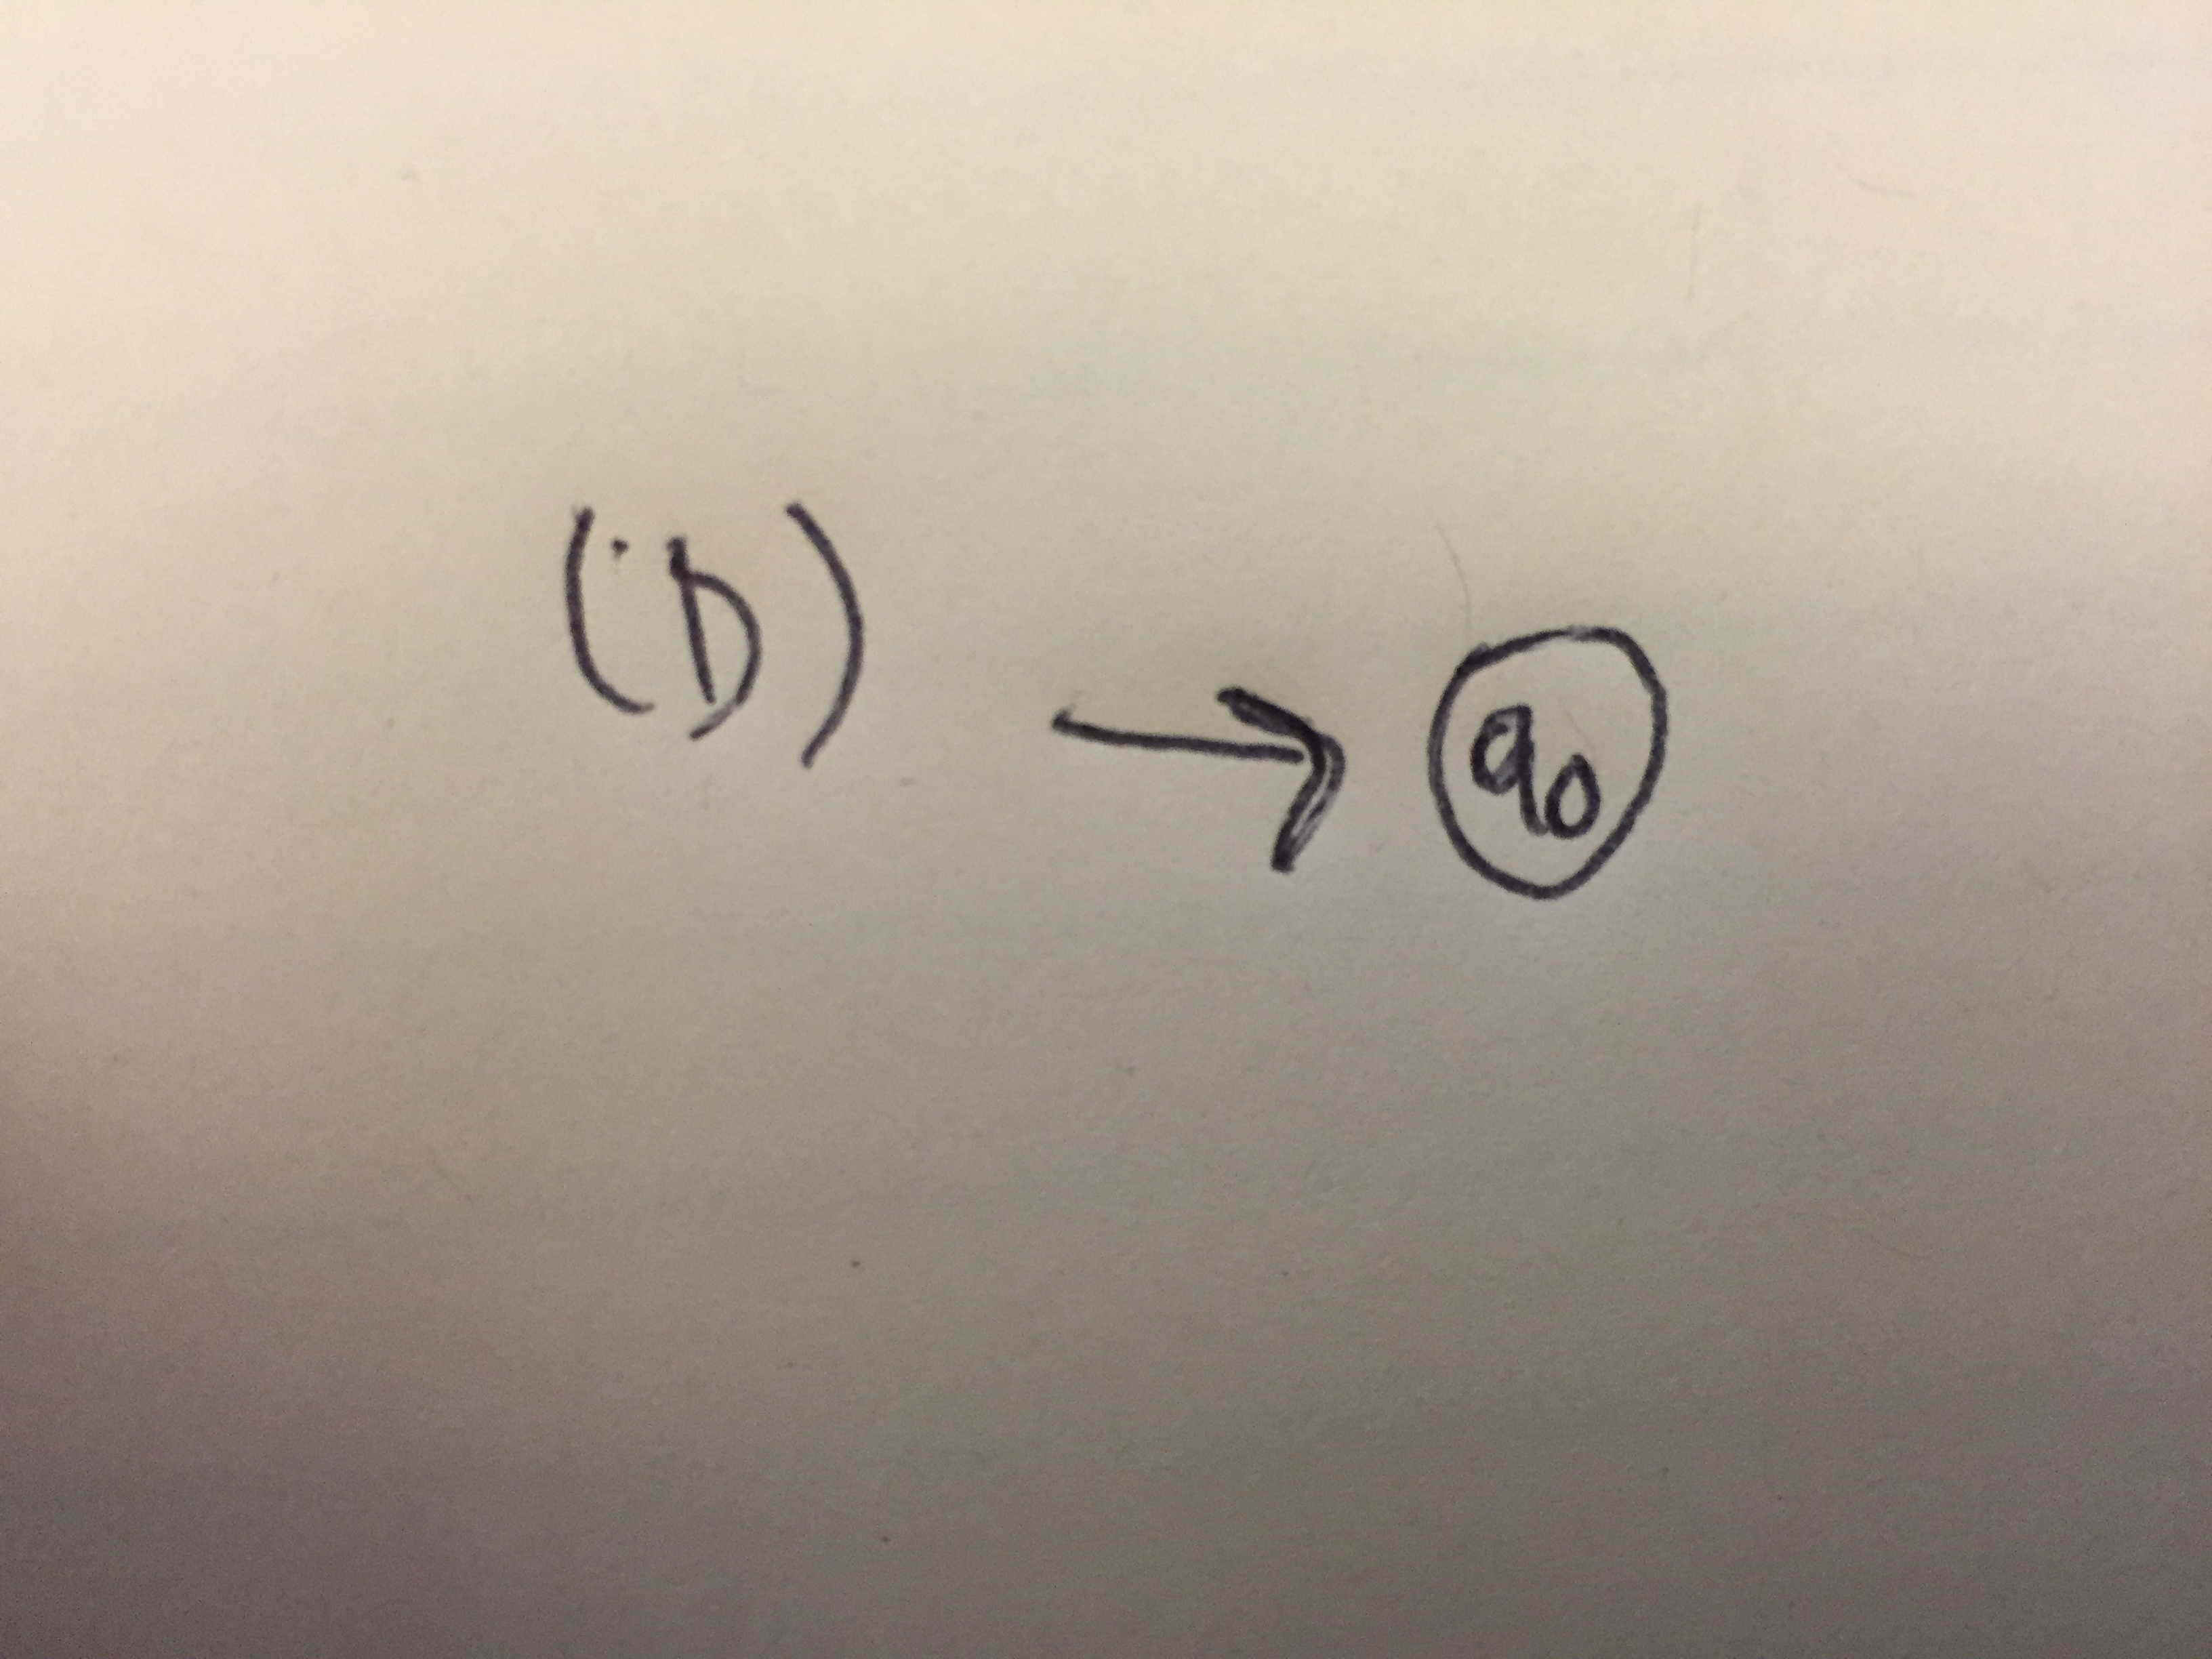
\includegraphics[width=15cm]{class16p1d}
\end{solution}

%% PROBLEM 2 %%
\problem We have a puzzle that looks like the following graph where we start on the black square in the center. Each move consists of moving to an adjacent square directly above, to the left, to the right, or below our current square.\\
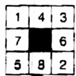
\includegraphics[width=2cm]{initial}
\subproblem What's the size of the state space after 1 move?
\subproblem What's the size of the state space after 2 moves?

\begin{solution}
\subsolution The size of the state space after 1 move is 4.
\subsolution The size of the state space after 2 moves is 8.\\
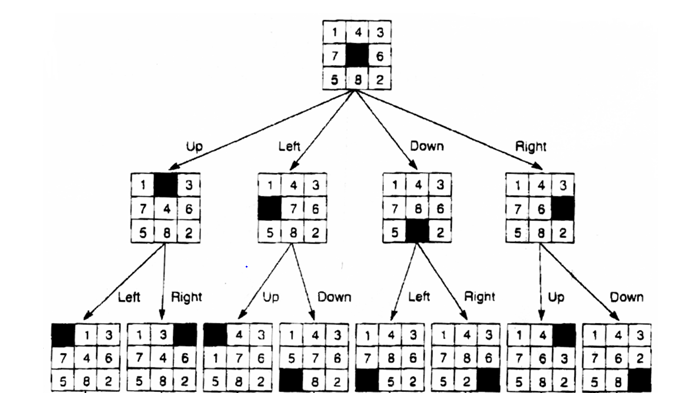
\includegraphics[width=12cm]{final8}
\end{solution}

%% PROBLEM 3 %%
\problem In this problem we will use loop invariants to prove the correctness property that $y=c$ (for $c>0$) after the following loop terminates.
\begin{itemize}
\item x=c; y=0;
\item while ($x>0$):
\subitem $x--$
\subitem $y$++
\end{itemize}
\subproblem Construct a loop invariant for the proof.
\subproblem Use induction to prove that the loop preserves the invariant.
\subproblem Use loop invariants to prove the correctness property that $y=c$ (for $c>0$) after the loop terminates.

\begin{solution}
\subsolution
\begin{itemize}
\item Let state set $S=N*N*N$ contain the values of $(x, y, c)$
\item $(x,y,c) \rightarrow (x-1, y+1, c)$  in each iteration of loop.
\item Let $P(x,y,n)\equiv$ $x+y=c$ 
\item $y$++
\end{itemize}
\subsolution
\begin{itemize}
\item Base case: loop invariant $x+y=c+0=c \rightarrow P(c,0,c)$ holds.
\item Induction step: \\
Assume loop invariant holds after $k$ iterations:\\
$x=c-k$; $y=k$;\\
after the ($k+1$)th iteration, $y=k+1$, $x=c-k-1$\\
And $x+y=k+1+c-k-1=c$\\
Therefore, the loop preserves the invariant $P(x,y,n)$.
\end{itemize}
\subsolution
After the final iteration $x=0$,\\
we also know that our loop invariant holds: $x+y=c$. Therefore, $y=c$.
\end{solution}

%% PROBLEM 4 %%
\problem (BONUS) Consider the following piece of code where $n$ is a positive integer:
\begin{itemize}
\item $y=0$; $i=0$
\item while ($i< n$):
\subitem $y += 2^i$
\subitem $i$++
\end{itemize}
\subproblem Compute the value of $y$ after the 0th, 1st, 2nd, and 3rd iterations. From these results, can you guess what the value of $y$ would be after the loop terminates?
\subproblem Use your result from (A) to construct a loop invariant.
\subproblem Use induction to prove that the loop preserves the invariant.
\subproblem Use the loop invariant to prove the correctness property that $y=c$ for $c>0$ after the loop terminates.

\begin{solution}
\subsolution
\begin{itemize}
\item iteration 0: $y_0=0=2^0-1$
\item iteration 1: $y_1=2^0=1=2^1-1$
\item iteration 2: $y_2=2^0+2^1=1+2=3=2^2-1$
\item iteration 3: $y_3=2^0+2^1+2^2=1+2+4=7=2^3-1$
\item iteration $n$: $y_n=2^0+2^1+2^2+...+2^{n-1}=2^n-1$
\end{itemize}
\subsolution
\begin{itemize}
\item Let state set S=$N*N*N$ contain the values of $(y, i, n)$
\item $(y,i,n) \rightarrow (y+2^i, i+1, n)$ for each iteration of the loop.
\item Let $P(y, i, n)\equiv y=2^i -1$ 
\end{itemize}
\subsolution
\begin{itemize}
\item Base case: i=0: $y_0=0=2^0-1 \rightarrow P(0,0,n)$ holds.
\item Induction step: \\
Assume that at the start of the $k$th iteration $y_k=2^k-1$\\
Then, at the start of the $(k+1)$th iteration we will have:\\
$y_{k+1}=y_k+2^k=2^k-1+2^k=2*2^k-1=2^{k+1}-1$ 

Q.E.D.
\end{itemize}
\subsolution
The loop terminates when $i=n$. Thus, after the loop finishes running we have: $y=2^{n}-1$
\end{solution}

\end{document}